% !TEX TS-program = pdflatex
% !TEX encoding = UTF-8 Unicode
% !TEX spellcheck = en_US

\documentclass[11pt]{article}
\usepackage[utf8]{inputenc} 
\usepackage{geometry}
\geometry{a4paper}
% \usepackage[german]{babel}
\usepackage{mathtools}
\usepackage{amsfonts,amsmath,amssymb,amsthm, amsbsy}
\usepackage{tikz}
\usetikzlibrary{arrows}
\usetikzlibrary{fit}
\usepackage{subfigure}
\tikzstyle{vertex}=[circle,fill=black!25,minimum size=20pt,inner sep=0pt]
\tikzstyle{selected vertex} = [vertex, fill=red!24]
\tikzstyle{edge} = [draw,thick,->]
\tikzstyle{weight} = []

\usepackage{graphicx}
\usepackage[parfill]{parskip}
\usepackage{booktabs} % for much better looking tables
\usepackage{array} % for better arrays (eg matrices) in maths
\usepackage{paralist} % very flexible & customisable lists (eg. enumerate/itemize, etc.)
\usepackage{verbatim} % adds environment for commenting out blocks of text & for better verbatim
\usepackage{subfig} % make it possible to include more than one captioned figure/table in a single float
\usepackage{amsfonts}
\usepackage{amsmath}
\usepackage{amsthm}
\usepackage{amssymb}
\usepackage{mathtools}
\usepackage{stmaryrd}
\usepackage{mathabx}
\usepackage[]{algorithm2e}
\usepackage{pdflscape}

\usepackage{proof}

\usepackage{pgf}
\usepackage{tikz}
\usetikzlibrary{matrix,positioning,automata,arrows,shapes,petri}
\tikzset{
place/.style={circle,thick,draw=black,minimum size=10mm},
transition/.style={rectangle,thick,draw=black,minimum width=3mm,inner ysep=5mm, fill=black}
}

\usepackage{xcolor}
\definecolor{secblue}{rgb}{0.18, 0.39, 0.77}
\definecolor{deepblue}{rgb}{0,0,0.5}
\definecolor{deepred}{rgb}{0.6,0,0}
\definecolor{deepgreen}{rgb}{0,0.5,0}

\usepackage{sectsty}
\allsectionsfont{\normalfont\sffamily\bfseries\color{secblue}}

%%% Aliases
\DeclarePairedDelimiter\floor{\lfloor}{\rfloor}
\DeclarePairedDelimiter\abs{\lvert}{\rvert}

% Command to declare a column vector. Param 1 is the dimension, then n elements follow
\newcount\colveccount
\newcommand*\colvec[1]{
        \global\colveccount#1
        \begin{pmatrix}
        \colvecnext
}
\def\colvecnext#1{
        #1
        \global\advance\colveccount-1
        \ifnum\colveccount>0
                \\
                \expandafter\colvecnext
        \else
                \end{pmatrix}
        \fi
}

\def\arraystretch{1.33}


\title{Concurrency Theory \\ Exercise Sheet 8}
\author{
	Franks, Billy Joe \\
	\texttt{b\_franks12@cs.uni-kl.de}
	\and 
	Kahraman, Kerem \\
	\texttt{keremkahraman@hotmail.de}
	\and 
	Bergsträßer, Pascal \\
	\texttt{p\_bergstra15@cs.uni-kl.de}
}

\newtheorem{theorem}{Satz}

\begin{document}
\maketitle
% !TeX root = root.tex
% !TeX spellcheck = en_US
\section{Weak Bisimulation}
\begin{align*}
& (\nu c)((?a.!c.0|?b.!c.0)&|?c.?c.P) \\
\equiv & (\nu c)(?a.(!c.0|?b.!c.0+?b.(?a.!c.0|!c.0))&|?c.?c.P)
\end{align*}
\begin{align*}
& (\nu c)(?a.(!c.0|?b.!c.0+?b.(?a.!c.0|!c.0))|?c.?c.P)&&&&\\
\equiv & (\nu c)(?a.(!c.0|?b.!c.0)|?c.?c.P&+& ?b.(?a.!c.0|!c.0))|?c.?c.P &+& ?c.R)\\
\equiv & (\nu c)(?a.(!c.0|?b.!c.0)|?c.?c.P)&+& (\nu c)(?b.(?a.!c.0|!c.0))|?c.?c.P) &+& (\nu c)(?c.R)\\
\equiv & (\nu c)(?a.(!c.0|?b.!c.0)|?c.?c.P)&+& (\nu c)(?b.(?a.!c.0|!c.0))|?c.?c.P) &+& 0\\
\equiv & (\nu c)(?a.(!c.0|?b.!c.0)|?c.?c.P)&+& (\nu c)(?b.(?a.!c.0|!c.0))|?c.?c.P) &&\\
\end{align*}

With some analog steps we reach

\begin{align*}
?a.(\nu c)((!c.0|?b.!c.0)|?c.?c.P)+?b.(\nu c)((?a.!c.0|!c.0))|?c.?c.P)
\end{align*}

We only consider one of the $+$ and ignore the $?a.$

\begin{align*}
&(\nu c)((!c.0|?b.!c.0)|?c.?c.P)\\
\equiv &(\nu c)((!c.(0|?b.!c.0)+?b.(!c.0|!c.0))|?c.?c.P)\\
\equiv &(\nu c)( ?b.(!c.0|!c.0|?c.?c.P) + (0|?b.!c.0|?c.P))\\
\equiv &?b.((\nu c)(!c.0|!c.0|?c.?c.P)) + (\nu c)(0|?b.!c.0|?c.P)
\end{align*}

With multiple steps ignoring resulting 0s we get from the left $+$, ignoring the $?b.$
\begin{align*}
&(\nu c)(!c.0|!c.0|?c.?c.P)\\
\equiv &(\nu c)(0|0|P)\\
\equiv &(\nu c) P\\
\equiv &P
\end{align*}

And the right $+$

\begin{align*}
&(\nu c)(0|?b.!c.0|?c.P)\\
\equiv &(\nu c)(?b.!c.0|?c.P)\\
\equiv &(\nu c)(?b.(!c.0|?c.P))\\
\equiv &?b.((\nu c)(!c.0|?c.P))\\
\equiv &?b.((\nu c)(0|P))\\
\equiv &?b.((\nu c) P)\\
\equiv &?b.P
\end{align*}

Both are equal and thus we finally get that the initial left side is equivalent to (we ignored the $?a.$ and the $?b.$ in the first of the two)

\begin{align*}
&?a.(\nu c)((!c.0|?b.!c.0)|?c.?c.P)\\
\equiv &?a.?b.P
\end{align*}

We can do the same analog for the right side and thus get

\begin{align*}
&(\nu c)((?a.!c.0|?b.!c.0)|?c.?c.P)\\
\equiv &?a.?b.P + ?b.?a.P
\end{align*}

Which is what was asked to prove.

\clearpage
% !TeX root = root.tex
% !TeX spellcheck = en_US
\section{Encoding Programs as Automaton}
\textbf{Task 1.} 
The following automata shows the example of a semaphore program for $P=3$ simultaneous programs and $n=2$ acquire permits.
\begin{figure}[h]
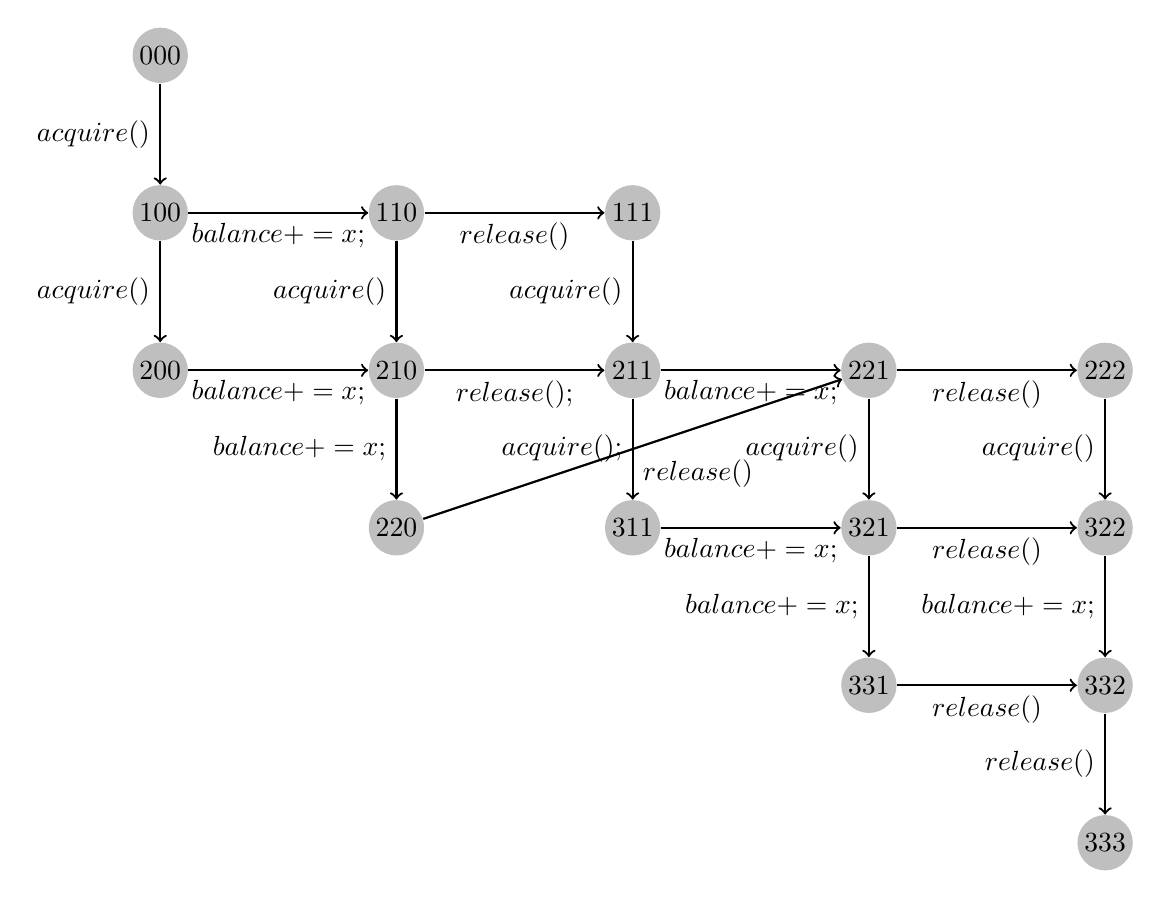
\begin{tikzpicture}[auto,swap]
    \foreach \pos/\name in {{(0,2)/000}, {(0,0)/100}, {(3,0)/110},{(6,0)/111},{(0,-2)/200},{(3,-2)/210},{(6,-2)/220},{(6,-2)/211},{(9,-2)/221},{(12,-2)/222},{(6,-4)/311},{(9,-4)/321},{(12,-4)/322},{(3,-4)/220},{(9,-6)/331},{(12,-6)/332},{(12,-8)/333}}
        \node[vertex] (\name) at \pos {$\name$};
    \foreach \source/ \dest /\weight in {000/100/acquire(), 100/200/acquire(),100/110/balance+=x;,200/210/balance+=x;,110/111/release(),210/211/release();,111/211/acquire(),211/311/acquire();,211/221/balance+=x;,221/222/release(),221/321/acquire(),321/322/release(),222/322/acquire(),311/321/balance+=x;,110/210/acquire(),210/220/balance+=x;,220/221/release(),321/331/balance+=x;,331/332/release(),332/333/release(),322/332/balance+=x;}
        \path[edge] (\source) -- node[weight] {$\weight$} (\dest);
\end{tikzpicture}
\end{figure}
\\
\textbf{Task 2.} According to the task a thread can use lock() an arbitrary amount of times. This makes the state space infinte and therefor the reentrant lock cannot be represented by an NFA. If there is a maximum amount $n$ of times lock() can be used the automaton will look like $n$ merged lock automatons.

\clearpage
% !TeX root = root.tex
% !TeX spellcheck = en_US
\section{Lossy Channel Systems with Test for Empty Channel}

\end{document}
